%!TEX root = ../thesis.tex
%*******************************************************************************
%*********************************** First Chapter *****************************
%*******************************************************************************

\chapter{Design - QSAR with SOAP-GP}
\section{Introduction}
Challenging though synthesis planning may be, at least it is fairly well-established and straightforward -- the difficulty in designing drug candidates, on the other hand, continues to be the scientific bottleneck in drug discovery. A key question is how to predict physical properties or bioactivity from molecular structure –- quantitative structure–activity relationships (QSAR) modelling. While statistical and machine learning (ML) approaches have been developed for QSAR since the 1970s, significant amount of innovation has occurred in the space of models -- from classical ML methods such as random forest and support vector machine, to the latest technologies based on deep neural networks. Central to any machine learning methodology is the way molecules are described within the model. Most methodologies to date treat a molecule as a 2D object -- a graph where the atoms are nodes and the bonds are edges. This leads to the extended connectivity fingerprint (ECFP) \cite{rogers2010extended} and more recent advances that extract the best possible representation of a 2D molecule graph using an end-to-end differentiable framework \cite{duvenaud2015convolutional}. 

Nonetheless, the physical mechanism that underlies biological activity is favourable interactions between local regions on the 3D surface of a molecule (pharmacophores) and residues in the receptor binding site. As such, one would expect that the 3D shape of the molecule would be a more appropriate input. Approaches that attempt to capture this such as Comparative Molecular Field Analysis \cite{cramer1988comparative,clark1990comparative} and Rapid Overlay of Chemical Structures \cite{rush2005shape} have been developed in the literature. However, those methods either require manual alignment \cite{cramer1988comparative,clark1990comparative} --  introducing bias -- or consider the similarity between the shapes of entire molecules \cite{masek1993molecular,rush2005shape}, overlooking the fact that it is often specific regions of the molecule that drive binding or determine physicochemical properties. Overcoming this limitation, one can coarse-grain the molecule into sites of salient interactions \cite{jenkins20043d}, but this requires prior insights on what are the important molecule-receptor interactions. Focusing on locality, Axen et al.~\cite{axen2017simple} developed an approach inspired by extended connectivity fingerprints, where the local 3D environments around each atom are mapped into a fixed length vector via hashing. However, this representation is lossy, and the process of folding into a fix length representation leads to different 3D environments being indistinguishable. (need to deal with this)

The problem of representing and comparing local atomic environments has received significant attention in the field of interpolating potential energy surfaces. Recent pioneering studies proposed a powerful mathematical formalism -- Smooth Overlap of Atomic Positions (SOAP) \cite{bartok2013representing}. The key idea is to first represent each atomic environment using a sum of Gaussian densities, then ensure rotational invariance by integrating over all rotations (analytically tractable using the mathematics of spherical harmonics), and finally compute molecular similarity between two molecules by the similarity between the atomic environments that are the most similar. SOAP has found success in cracking challenging problems in materials science such as the phase behavior and defect structure of carbon \cite{caro2018growth}, boron \cite{deringer2018data} and silicon \cite{bartok2018machine}. Although SOAP has become the workhorse in computational physics, it has not been extensively tested and deployed in cheminformatics. Some examples of ligand-based virtual screening using SOAP \cite{bartok2017machine} have been reported, but a systematic exploration of the utility of SOAP as a general purpose 3D QSAR method has thus far not been done. 

% In this chapter, we will first describe a SOAP ML model (SOAP-GP) and show that it can exceed state-of-the-art graph neural networks in raw performance and data efficiency on regression tasks despite having very few hyperparameters, even in challenging scaffold splits which address dataset bias \cite{wallach2018most,sieg2019need}. We will then show that the uncertainties predicted using SOAP-GP are well-calibrated. Finally, we show that combining SOAP-GP and graph neural network models together as an ensemble further outperforms the state-of-the-art. (need to rewrite this, include something about the non-distinguishability in performance between representations)

In this chapter, we will first describe an ML model utilising SOAP descriptors (SOAP-GP) and show that it can comfortably compete and outperform traditional fingerprint-based approaches as well as state-of-the-art graph neural networks on predicting binding affinity, even in challenging scaffold splits which address dataset bias \cite{wallach2018most,sieg2019need}. That being said, we emphasize that we are not advocating for SOAP-GP to become the new paradigm in cheminformatics QSAR. We instead argue that one should exploit the richness of chemical featurisation by combining ML models using different molecular representations rather than relying on any one particular method. We justify this claim by demonstrating that an ensemble of models with different representations outperform equivalently-sized ensembles of the same model/representation.

The work in this chapter is a continuation of my MSci research project from the year before. A paper based on prior results had been submitted to the Journal of Medicinal Chemistry, and will shortly be resubmitted after taking into account comments from reviewers. All code used in this chapter can be found in the GitHub repo \texttt{soapgp}  \cite{McCorkindale2020SOAPGP}.

\section{Methods}\label{sec:experiment}

\subsection{SOAP-GP}
In the SOAP framework \cite{bartok2013representing}, the local atomic environment of an atom $\textbf{x}$ is represented by the sum of element-specific Gaussian densities centered on the positions of neighbourhood atoms. The ``similarity'' between two atomic environments is given by $k(\textbf{x}_{i}, \textbf{x}_{j}) = \textbf{x}_{i} \cdot \textbf{x}_{j}$, where the similarity function $k$ between environments represents the overlap of these neighbourhood densities integrated over all rotations (normalized so that self-similarity is unity). Using spherical harmonics and radial basis functions, this integral can be analytically computed as a truncated sum of coefficients -- the vector of these coefficients forms the descriptor $\textbf{x}$. This construction is invariant to rotations, translations, and permutations, and thus alignment-free. 
Please provide more details about the loss of resolution due to integrating over all
rotations. This means that the per-atom-environment comparisons could be nonphysical
in the sense that one maximal “alignment” is not possible in the context of another.

To find the geometric similarity between two molecules $A$ and $B$ (Fig \ref{fig:soap}), the local similarities of the best possible pairing of the atomic environments in $A$ and $B$ are used:
\begin{equation}\label{eq:rematch}
    K(A,B) = \displaystyle\sum_{\substack{i \in A\\ j \in B}}P_{ij}k(\textbf{x}_{i}, \textbf{x}_{j})
\end{equation}
where $P_{ij}$ is $i-j$th element of the permutation matrix $P$ that maximises $K$. This can be expressed as an optimal assignment problem and computed efficiently using an entropy-regularization approach, and is known as the ``REMatch'' similarity kernel~\cite{de2016comparing}. The `distance' between $A$ and $B$, which can be understood to be a measure of the geometric difference between these two molecules, can then be easily evaluated as

\begin{equation}\label{eq:distance}
    d(A, B) = \sqrt{2 - 2K(A, B)}
\end{equation}

\begin{figure}[!h] % !h ~ force here, t ~ top, b ~ bottom, p ~ separate page
\centering
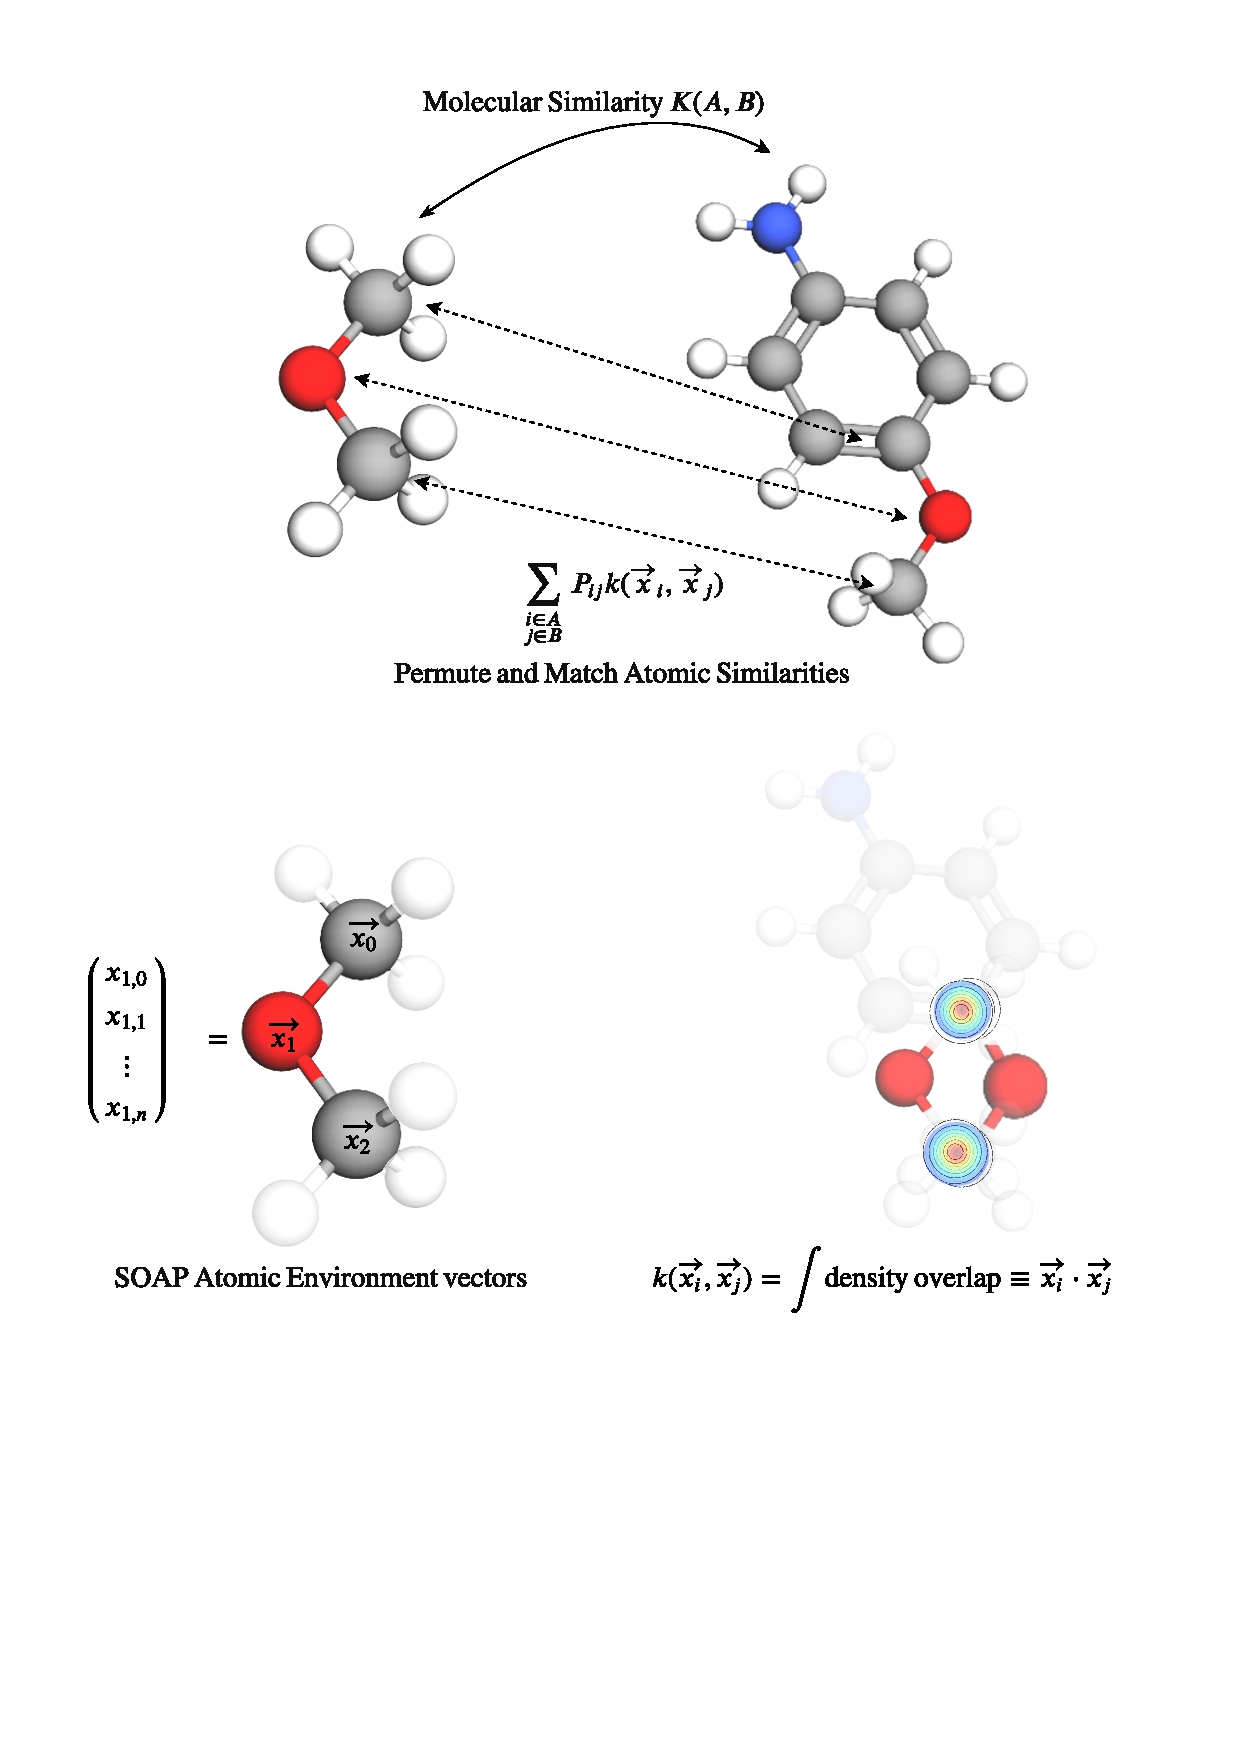
\includegraphics[width=\textwidth]{Chapter2/Figs/SOAP.pdf}
\caption{\label{fig:soap} An illustration of how molecular similarity is defined by permuting and maximising the similarity of atomic environments between molecules.}
\end{figure}

The SOAP framework thus allows us to represent differences in three-dimensional molecular shape between individual molecules in a principled, alignment-free manner as a singular metric. Since the binding of ligands to proteins strongly depends on the three-dimensional interactions between the ligand and the receptor binding site, there is reason to expect that such a precise measure of molecular shape could act as an informative descriptor for predicting bioactivity.

This method differs in approach from conventional QSAR methods in that no explicit chemistry descriptors (eg bonding, hybridization, aromaticity) are used at all in the featurisation of a molecule. Instead, chemical information is implicitly learned from the conformational shape of the molecule, from the coordinates of the atoms relative to one another, and completely encoded in the form of a numerical distance metric.

Such an approach naturally lends itself into the framework of kernel-based machine learning methods. Well-known example of such methods are Gaussian Process Regression~\cite{rasmussen2005gp} (GP) models, which we implement using the Mat{\'e}rn kernel. We refer to GP models utilizing SOAP features as SOAP-GP (Fig \ref{fig:soapgp}). 

GP Regression is a Bayesian ML method which searches over a probabilistic distribution of functions of functions which could model the data. The kernel $K(X_{i},X_{j})$ between data points is used as the covariance of the prior distribution over functions, and the training data is used to construct a likelihood. With Bayes' theorem this defines a posterior distribution for prediction. The model is trained by optimizing the kernel hyperparameters in order to maximise the marginal likelihood of the distribution of functions which model the data. 

To incorporate smoothness and differentiability into the GP kernel in order assist in the learning of the model, we augment the REMatch distance $d(A,B)$ (Eq.~\ref{eq:distance}) with the $\nu=\frac{3}{2}$ Mat$\acute{\textrm{e}}$rn kernel $K^{\dagger}(A,B)$:
\begin{equation}
    K^{\dagger}(A,B) = \sigma^{2}\Big( 1+\frac{\sqrt{3}d}{\rho}\Big)\exp{\Big(-\frac{\sqrt{3}d}{\rho}\Big)}
\end{equation}
where $\sigma$ and $\rho$ are the kernel hyperparameters (both initialised at unity) to be optimized. 

\begin{figure}[!h] % !h ~ force here, t ~ top, b ~ bottom, p ~ separate page
\centering
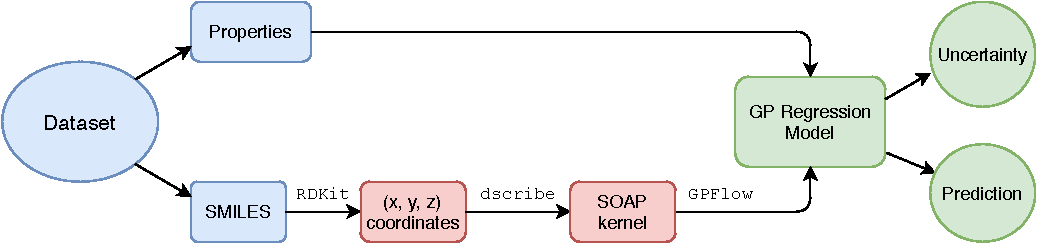
\includegraphics[width=\textwidth]{Chapter2/Figs/SOAPGP-horizontal.pdf}
\caption{\label{fig:soapgp} An overview of the SOAP-GP model implementation.}
\end{figure}

Computationally, SMILES strings of molecules are converted into $(x,y,z)$ atomic coordinates using the ETKDG conformer generation method (cite) implemented in \texttt{RDKit} \cite{rdkit}. Only one conformer is generated -- how one would incorporate multiple conformers and the fact that only one conformer is needed to achieve good predictive performance is discussed later. SOAP descriptors and kernels were computed from the resultant atomic coordinates using the \texttt{soapxx} and \texttt{dscribe} packages \cite{soapxx,dscribe}, with the basis function parameters $ n_{max}=12, l_{max}=8$. Two sets of SOAP descriptors with $r_{cut}=3.0\textup{\AA}, \sigma=0.2\textup{\AA}$ and $r_{cut}=6.0\textup{\AA}, \sigma=0.4\textup{\AA}$ were evaluated and concatenated for each molecule. For the REMatch kernel, the entropy regularization parameter $\alpha$ was set to $0.5$ with a convergence threshold of $10^{-6}$. The GP model itself was implemented using \texttt{GPFlow}.

%The relatively large value of $\alpha$ was chosen to make the resultant kernel intermediate between the average and best-match molecular kernels~\cite{de2016comparing}. This was motivated by the fact that the average kernel was shown to be an appropriate choice for modelling extensive properties (those that can be decomposed into atomic contributions), while the best-match kernel performs better for intensive properties~\cite{bartok2018machine}. Choosing an intermediate value of $\alpha$ is a compromise of the two approaches, and allows the model to better generalise to modelling different properties.   

\subsection{Comparative models}
The performance of our model was compared directly with that of several others which use representations of differing dimensionality and complexity. The intention of this exercise is not to establish an authoritative benchmark of QSAR model architectures by any means, merely as an illustration of how SOAP-GP compares to representative example models which utilise particular molecular featurisations. Indeed, SOAP itself is merely one example of the many ways in which those in the field of materials science seek to precisely describe atomic and crystal structures (eg atom-centered symmetry functions \cite{Behler2011, Faber2018}, many-body tensor representations \cite{huo2017unified}).

The industry standard approach for representing molecules is to use the extended connectivity fingerprint (ECFP), which considers molecules as 2D graphs and encodes the topological structural features of a molecule into a fixed-length binary bit string. ECFPs are a popular similarity search tool in drug discovery as the distance between two molecules can be simply defined as the Tanimoto distance between the bit strings \cite{Todeschini2012tanimoto}. We implement ECFPs in a random forest model (ECFP-RF), which is an established benchmark model for QSAR tasks.

An extension of ECFPs is to consider molecules as 3D structures instead of molecular graphs, which leads to the extended three-dimensional fingerprint (E3FP) \cite{Axen17e3fp}. The logic behind such an approach is that the 3D fingerprints are better able to encode stereochemistry and include information on the relationship between atoms close in space but distant in bond connectivity. The E3FP approach only considers radial distances between atoms in its featurisation, while SOAP features also encode angular information. Just like ECFPs, the similarity between two molecules can be calculated using the Tanimoto distance between their E3FP fingerprints.

For E3FPs there is no standard model implementation - both random forest and Gaussian Process models were attempted and the GP models on average performed better so we from hereon utilise E3FPs in a GP framework (E3FP-GP) with the Mat{\'e}rn kernel in an identical fashion as the SOAP-GP except that the Tanimoto distances between molecular fingerprints are used in place of the SOAP REMatch distance. The difference performance can be isolated to the quality of the molecular distance measures -- this would illustrate the importance of including angular information in featurising molecular shape.

Last but not least, we also consider the Directed Message Passing Neural Network (DMPNN) model~\cite{yang2019chemprop}, a state-of-the-art graph neural network which uses 2D molecular graphs explicitly encoding atomic and bond properties such as formal charge and conjugation as input features, usually as one-hot vectors. In graph neural networks, atom and bond features are combined with those of their neighbours via message-passing and convolutional embedding to construct a learnt global descriptor of a molecule, which is then passed through a neural network for property prediction. Graph neural networks have been gaining popularity in the cheminformatics community for property prediction \cite{Gilmer17mpnn, Feinberg18potentialnet}, and most recently the DMPNN model was utilised in a successful landmark deep learning search for novel antibiotics \cite{stokes2020antibiotic}. 

ECFP fingerprints were generated with a radius of 3 and 1024 bits using \texttt{RDKit}, while E3FP fingerprints also with 1024 bits were generated using the \texttt{e3fp} package \cite{Axen17e3fp}. The DMPNN model was implemented using the \texttt{chemprop} package. The training procedure regarding the molecular features used as well as the initial hyperparameter optimization was done following the guidelines from \cite{yang2019chemprop}.

\subsection{Datasets}\label{subsec:datasets}
We used IC50 datasets for 24 diverse protein targets extracted from ChEMBL which have been previously investigated in several screening and modelling studies \cite{Bender2018, Bender2019} . IC50 measures the concentration of a compound required for the inhibition of a target to drop by 50\% - the IC50 (or pIC50) values are a direct metric of ligand-protein binding affinity, and modelling these values are thus a suitable challenge for comparing QSAR models. We further filter the datasets as we found that they contained many large compounds such as glycans which are beyond the scope of small molecule drug discovery. We only keep molecules with molecular weight below 500 daltons (as per Lipinski's rules) which reduces the datasets by 19\% on average (Table~\ref{table:bender_datasets}). experimental error

\begin{table}[!h]
\caption{ChEMBL IC50 bioactivity data used in this study}
\centering
\label{table:bender_datasets}
\begin{tabular}{lcc}
\toprule
Target & Initial Length & Post-Filter Length \\ 
\midrule
A2a & 203 & 166\\
ABL1 & 773 & 536\\
Acetylcholinesterase & 3159 & 2491\\
Aurora-A & 2125 & 1612\\
B-raf & 1730 & 824\\
Cannabinoid & 1116 & 820\\
Carbonic & 603 & 556\\
Caspase & 1606 & 1362\\
Coagulation & 1700 & 862\\
COX-1 & 1343 & 1278\\
COX-2 & 2855 & 2704\\
Dihydrofolate & 584 & 548\\
Dopamine & 479 & 405\\
Ephrin & 1740 & 1716\\
erbB1 & 4868 & 3598\\
Estrogen & 1705 & 1546\\
Glucocorticoid & 1447 & 1077\\
Glycogen & 1757 & 1655\\
HERG & 5207 & 4042\\
JAK2 & 2655 & 2252\\
LCK & 1352 & 954\\
Monoamine & 1379 & 1344\\
opioid & 840 & 611\\
Vanilloid & 1923 & 1656\\
\bottomrule
\end{tabular}
\end{table}

For SOAP-GP, ECFP-RF, and E3FP-GP, the datasets are split 80/20 into train/test sets and for the DMPNN models the split is 70/10/20 for train/validation/test sets. The random split results are given as the mean results from 3 runs each with 5-fold cross validation.

Besides random splitting, we also evaluate on these datasets using scaffold split, where molecules are binned by Murcko scaffold (evaluated using \texttt{RDKit}). This method of splitting better simulates the real-life drug discovery cycle where prior activity data only exists for a class of chemical compounds that are different from those that are being evaluated, in other words posing a greater extrapolation challenge. Bins larger than half of the required test set size are placed in the training/validation set and all remaining bins are distributed randomly such that the required train/test split sizes are met. The scaffold split results are given as the mean results from 15 runs using different random seeds for the distribution of scaffolds.

\renewcommand{\arraystretch}{1.5}
\begin{table}
  \caption{pIC50 Random Split RMSE Results - the lowest RMSE for each dataset are bolded.} %(include R2?)
  \label{tbl:rand}
  \begin{tabular}{@{\extracolsep{4pt}}lrrrrr} 
    \hline 
    & \multicolumn{4}{c}{Random Split}\\
    \cline{2-5}
    Dataset & \multicolumn{1}{c}{ECFP-RF} & \multicolumn{1}{c}{E3FP-GP} & \multicolumn{1}{c}{DMPNN} & \multicolumn{1}{c}{SOAP-GP}\\
    \hline
    \hline
    A2a & $ 0.839\pm0.030 $& $ \textbf{0.793}\pm\textbf{0.034} $ & $ 0.993 \pm 0.062 $ & $ 0.924\pm0.064 $\\
    ABL1 & $ 0.848\pm0.018 $ & $ 0.843\pm0.019 $ & $ 0.965 \pm 0.030 $ & $ \textbf{0.798}\pm\textbf{0.017}$\\
    AChE & $ 0.784\pm0.006 $ & $ 0.868\pm0.007 $ & $ 0.783 \pm 0.011 $ & $ \textbf{0.761}\pm\textbf{0.009} $ \\
    Aurora-A & $ \textbf{0.830}\pm\textbf{0.010} $ & $ 0.900\pm0.008 $ & $ 0.842 \pm 0.008 $ & $ 0.844\pm0.009 $ \\
    B-raf & $ \textbf{0.712}\pm\textbf{0.008} $ & $ 0.786\pm0.008 $ & $0.778 \pm 0.010 $ & $ 0.720\pm0.008 $ \\
    Cannabinoid & $ 0.747\pm0.015 $ & $ 0.800\pm0.011 $ & $0.845 \pm 0.019$ & $ \textbf{0.716}\pm\textbf{0.011} $\\
    Carbonic & $ \textbf{0.659}\pm\textbf{0.016} $ & $ 0.670\pm0.013 $ & $0.702 \pm 0.023$ & $ 0.839\pm0.095 $ \\
    Caspase & $ \textbf{0.587}\pm\textbf{0.008} $ & $ 0.662\pm0.009 $ & $0.597 \pm 0.012$ & $ 1.096\pm0.061 $ \\
    Coagulation & $ \textbf{0.909}\pm\textbf{0.010}$ & $ 1.010\pm0.009 $ & $1.019 \pm 0.022$ & $ 0.984\pm0.037 $\\
    COX-1 & $ 0.729\pm0.013 $ & $ 0.744\pm0.013 $ & $0.732 \pm 0.011$ & $ \textbf{0.706}\pm\textbf{0.013} $ \\
    COX-2 & $ 0.790\pm0.007 $ & $ 0.826\pm0.007 $ & $0.804 \pm 0.012$ & $ \textbf{0.762}\pm\textbf{0.007} $\\
    Dihydrofolate & $ \textbf{0.799}\pm\textbf{0.025} $ & $ 0.849\pm0.019 $ & $0.890 \pm 0.023$ & $ 0.811\pm0.021 $ \\
    Dopamine & $ \textbf{0.747}\pm\textbf{0.013} $ & $ 0.816\pm0.014 $ & $0.921 \pm 0.020$ & $ 0.777\pm0.017 $ \\
    Ephrin & $ 0.722\pm0.011 $ & $ 0.749\pm0.007 $ & $0.719 \pm 0.009$ & $ \textbf{0.701}\pm\textbf{0.008} $\\
    erbB1 & $ \textbf{0.756}\pm\textbf{0.003} $ & $ 0.818\pm0.005 $ & $0.748 \pm 0.010$ & $ 0.772\pm0.003 $ \\
    Estrogen & $ 0.691\pm0.005 $ & $ 0.697\pm0.005 $ & $0.670 \pm 0.007$ & $ \textbf{0.633}\pm\textbf{0.007} $\\
    Glucocorticoid & $ \textbf{0.612}\pm\textbf{0.010} $ & $ 0.663\pm0.008 $ & $0.691 \pm 0.008$ & $ 0.613\pm0.007 $ &\\
    Glycogen & $ \textbf{0.743}\pm\textbf{0.007} $ & $ 0.788\pm0.008 $ & $0.806 \pm 0.009$ & $ 0.769\pm0.006 $ \\
    HERG & $ 0.610\pm0.006 $ & $ 0.679\pm0.005 $ & $0.615 \pm 0.007$ & $ \textbf{0.569}\pm\textbf{0.005} $\\
    JAK2 & $ \textbf{0.672}\pm\textbf{0.007} $ & $ 0.737\pm0.007 $ & $0.719 \pm 0.007$ & $ 0.683\pm0.009 $ \\
    LCK & $ 0.829\pm0.010 $ & $ 0.867\pm0.012 $ & $0.918 \pm 0.021$ & $ \textbf{0.827}\pm\textbf{0.010} $ \\
    Monoamine & $ \textbf{0.676}\pm\textbf{0.007} $ & $ 0.680\pm0.008 $ & $0.724 \pm 0.012$ & $ 0.680\pm0.009 $ \\
    opioid & $ 0.729\pm0.011 $ & $ 0.781\pm0.018 $ & $0.748 \pm 0.020$ & $ \textbf{0.692}\pm\textbf{0.015} $\\
    Vanilloid & $ 0.724\pm0.006 $ & $ 0.774\pm0.006 $ & $0.744 \pm 0.008$ & $ \textbf{0.720}\pm\textbf{0.006} $ \\
    \hline
    \end{tabular}
\end{table}

\begin{table} 
\begin{tabular}{@{\extracolsep{4pt}}lrrrrr}
\hline
  %\caption{RMSE Results - E3FP 1024bits, ECFP 2048 bits}
    & \multicolumn{4}{c}{Scaffold Split}\\
    \cline{2-5}
    Dataset & \multicolumn{1}{c}{ECFP-RF} & \multicolumn{1}{c}{E3FP-GP} & \multicolumn{1}{c}{DMPNN} & \multicolumn{1}{c}{SOAP-GP}\\
    \hline
    \hline
    A2a & $ 1.113\pm0.087 $ & $ 1.134\pm0.128 $ & $1.434 \pm 0.194$ & $ \textbf{1.028}\pm\textbf{0.065} $ \\
    ABL1 & $ \textbf{0.933}\pm\textbf{0.036} $ & $ 0.971\pm0.047 $ & $1.069 \pm 0.043$ & $ 0.951\pm0.050 $ \\
    AChE & $ 0.990\pm0.023 $ & $ 1.045\pm0.025 $ & $0.994 \pm 0.030$ & $ \textbf{0.952}\pm\textbf{0.022} $ \\
    Aurora-A & $ \textbf{0.928}\pm\textbf{0.025} $ & $ 1.011\pm0.021 $ & $0.953 \pm 0.029$ & $ 0.942\pm0.017 $ \\
    B-raf & $ 0.866\pm0.038 $ & $ 0.916\pm0.038 $ & $0.959 \pm 0.032$ & $ \textbf{0.841}\pm\textbf{0.035} $ \\
    Cannabinoid & $ 0.874\pm0.026 $ & $ 0.943\pm0.028 $ & $0.967 \pm 0.027$ & $ \textbf{0.827}\pm\textbf{0.022} $ \\
    Carbonic & $ \textbf{0.682}\pm\textbf{0.032} $ & $ 0.816\pm0.044 $ & $0.809 \pm 0.060$ & $ 0.689\pm0.049 $ \\
    Caspase & $ \textbf{0.721}\pm\textbf{0.040} $ & $ 0.764\pm0.027 $ & $0.770 \pm 0.025$ & $ 0.922\pm0.063 $ \\
    Coagulation & $ 0.996\pm0.014 $ & $ 1.076\pm0.023 $ & $1.100 \pm 0.025$ & $ \textbf{0.989}\pm\textbf{0.025} $ \\
    COX-1 & $ 0.793\pm0.017 $ & $ 0.789\pm0.014 $ & $\textbf{0.768} \pm \textbf{0.008}$ & $ 0.781\pm0.009 $ \\
    COX-2 & $ 1.008\pm0.039 $ & $ 1.009\pm0.031 $ & $1.010 \pm 0.037$ & $ \textbf{0.960}\pm\textbf{0.033} $ \\
    Dihydrofolate & $\textbf{0.914}\pm\textbf{0.058} $ & $ 0.938\pm0.051 $ & $1.012 \pm 0.044$ & $ 0.967\pm0.057 $ \\
    Dopamine & $ \textbf{0.869}\pm\textbf{0.020} $ & $ 0.882\pm0.018 $ & $0.940 \pm 0.020$ & $ 0.894\pm0.020 $ \\
    Ephrin & $ \textbf{0.881}\pm\textbf{0.018} $ & $ 0.908\pm0.028 $ & $0.904 \pm 0.025$ & $ 0.882\pm0.021 $ \\
    erbB1 & $ 0.888\pm0.013 $ & $ 0.947\pm0.012 $ & $\textbf{0.864} \pm \textbf{0.010}$ & $ 0.891\pm0.007 $\\
    Estrogen & $ 0.795\pm0.018 $ & $ 0.786\pm0.015 $ & $0.744 \pm 0.014$ & $ \textbf{0.708}\pm\textbf{0.011} $ \\
    Glucocorticoid & $ 0.742\pm0.023 $ & $ 0.790\pm0.024 $ & $0.859 \pm 0.022$ & $ \textbf{0.738}\pm\textbf{0.014} $ \\
    Glycogen & $ \textbf{0.869}\pm\textbf{0.021}$ & $ 0.910\pm0.022 $ & $0.963 \pm 0.022$ & $ 0.906\pm0.020 $ \\
    HERG & $ 0.690\pm0.018 $ & $ 0.747\pm0.021 $ & $0.706 \pm 0.023$ & $ \textbf{0.656}\pm\textbf{0.018} $ \\
    JAK2 & $ 0.746\pm0.010 $ & $ 0.803\pm0.013 $ & $0.783 \pm 0.019$ & $ \textbf{0.738}\pm\textbf{0.021} $ \\
    LCK & $ \textbf{0.909}\pm\textbf{0.014} $ & $ 0.954\pm0.018 $ & $1.056 \pm 0.030$ & $ 0.918\pm0.012 $ \\
    Monoamine & $ 0.818\pm0.022 $ & $ \textbf{0.813}\pm\textbf{0.023} $ & $0.927 \pm 0.030$ & $ 0.817\pm0.023 $\\
    opioid & $ 0.781\pm0.032 $ & $ 0.797\pm0.031 $ & $0.811 \pm 0.028$ & $ \textbf{0.747}\pm\textbf{0.021} $ \\
    Vanilloid & $ 0.770\pm0.018 $ & $ 0.814\pm0.018 $ & $0.826 \pm 0.026$ & $ \textbf{0.762}\pm\textbf{0.015} $ \\
    \hline
    \end{tabular}
\end{table}
% \begin{table}
%   \caption{pIC50 Random Split RMSE Results - bolded entries indicate statistical significance} %(include R2?)
%   \label{tbl:rand}
%   \begin{tabular}{@{\extracolsep{4pt}}lrrrrr} 
%     \hline 
%     & \multicolumn{4}{c}{Random Split}\\
%     \cline{2-5}
%     Dataset & \multicolumn{1}{c}{ECFP-RF} & \multicolumn{1}{c}{E3FP-GP} & \multicolumn{1}{c}{DMPNN} & \multicolumn{1}{c}{SOAP-GP}\\
%     \hline
%     \hline
%     A2a & $ 0.839\pm0.030 $& $ 0.793\pm0.034 $ & $ 0.967\pm0.029 $ & $ 0.924\pm0.064 $\\
%     ABL1 & $ 0.848\pm0.018 $ & $ 0.843\pm0.019 $ & $ 0.948\pm0.014 $ & $ \textbf{0.798}\pm\textbf{0.017}$\\
%     AChE & $ 0.784\pm0.006 $ & $ 0.868\pm0.007 $ & $ 0.754\pm0.007 $ & $ 0.761\pm0.009 $ \\
%     Aurora-A & $ 0.830\pm0.010 $ & $ 0.900\pm0.008 $ & $ 0.827\pm0.004 $ & $ 0.844\pm0.009 $ \\
%     B-raf & $ 0.712\pm0.008 $ & $ 0.786\pm0.008 $ & $ 0.769\pm0.010 $ & $ 0.720\pm0.008 $ \\
%     Cannabinoid & $ 0.747\pm0.015 $ & $ 0.800\pm0.011 $ & $ 0.825\pm0.011 $ & $ \textbf{0.716}\pm\textbf{0.011} $\\
%     Carbonic & $ 0.659\pm0.016 $ & $ 0.670\pm0.013 $ & $ 0.688\pm0.013 $ & $ 0.839\pm0.095 $ \\
%     Caspase & $ 0.587\pm0.008 $ & $ 0.662\pm0.009 $ & $ 0.599\pm0.006 $ & $ 1.096\pm0.061 $ \\
%     Coagulation & $ \textbf{0.909}\pm\textbf{0.010}$ & $ 1.010\pm0.009 $ & $ 0.999\pm0.011 $ & $ 0.984\pm0.037 $\\
    % COX-1 & $ 0.729\pm0.013 $ & $ 0.744\pm0.013 $ & $ 0.718\pm0.007 $ & $ 0.706\pm0.013 $ \\
    % COX-2 & $ 0.790\pm0.007 $ & $ 0.826\pm0.007 $ & $ 0.788\pm0.007 $ & $ \textbf{0.762}\pm\textbf{0.007} $\\
    % Dihydrofolate & $ \textbf{0.799}\pm\textbf{0.025} $ & $ 0.849\pm0.019 $ & $ 0.896\pm0.016 $ & $ 0.811\pm0.021 $ \\
    % Dopamine & $ \textbf{0.747}\pm\textbf{0.013} $ & $ 0.816\pm0.014 $ & $ 0.895\pm0.012 $ & $ 0.777\pm0.017 $ \\
    % Ephrin & $ 0.722\pm0.011 $ & $ 0.749\pm0.007 $ & $ 0.715\pm0.005 $ & $ \textbf{0.701}\pm\textbf{0.008} $\\
    % erbB1 & $ 0.756\pm0.003 $ & $ 0.818\pm0.005 $ & $ \textbf{0.715}\pm\textbf{0.004} $ & $ 0.772\pm0.003 $ \\
    % Estrogen & $ 0.691\pm0.005 $ & $ 0.697\pm0.005 $ & $ 0.675\pm0.005 $ & $ \textbf{0.633}\pm\textbf{0.007} $\\
    % Glucocorticoid & $ \textbf{0.612}\pm\textbf{0.010} $ & $ 0.663\pm0.008 $ & $ 0.694\pm0.008 $ & $ 0.613\pm0.007 $ &\\
    % Glycogen & $ 0.743\pm0.007 $ & $ 0.788\pm0.008 $ & $ 0.788\pm0.006 $ & $ 0.769\pm0.006 $ \\
%     HERG & $ 0.610\pm0.006 $ & $ 0.679\pm0.005 $ & $ 0.597\pm0.003 $ & $ \textbf{0.569}\pm\textbf{0.005} $\\
%     JAK2 & $ 0.672\pm0.007 $ & $ 0.737\pm0.007 $ & $ 0.702\pm0.005 $ & $ 0.683\pm0.009 $ \\
%     LCK & $ 0.829\pm0.010 $ & $ 0.867\pm0.012 $ & $ 0.901\pm0.010 $ & $ 0.827\pm0.010 $ \\
%     Monoamine & $ 0.676\pm0.007 $ & $ 0.680\pm0.008 $ & $ 0.703\pm0.007 $ & $ 0.680\pm0.009 $ \\
%     opioid & $ 0.729\pm0.011 $ & $ 0.781\pm0.018 $ & $ 0.736\pm0.011 $ & $ \textbf{0.692}\pm\textbf{0.015} $\\
%     Vanilloid & $ 0.724\pm0.006 $ & $ 0.774\pm0.006 $ & $ 0.732\pm0.005 $ & $ 0.720\pm0.006 $ \\
%     \hline
%     \end{tabular}
% \end{table}

% \begin{table} 
% \begin{tabular}{@{\extracolsep{4pt}}lrrrrr}
% \hline
%   %\caption{RMSE Results - E3FP 1024bits, ECFP 2048 bits}
%     & \multicolumn{4}{c}{Scaffold Split}\\
%     \cline{2-5}
%     Dataset & \multicolumn{1}{c}{ECFP-RF} & \multicolumn{1}{c}{E3FP-GP} & \multicolumn{1}{c}{DMPNN} & \multicolumn{1}{c}{SOAP-GP}\\
%     \hline
%     \hline
%     A2a & $ 1.113\pm0.087 $ & $ 1.134\pm0.128 $ & $ 1.354\pm0.234 $ & $ 1.028\pm0.065 $ \\
%     ABL1 & $ 0.933\pm0.036 $ & $ 0.971\pm0.047 $ & $ 1.068\pm0.050 $ & $ 0.951\pm0.050 $ \\
%     AChE & $ 0.990\pm0.023 $ & $ 1.045\pm0.025 $ & $ 0.981\pm0.031 $ & $ 0.952\pm0.022 $ \\
    % Aurora-A & $ 0.928\pm0.025 $ & $ 1.011\pm0.021 $ & $ 0.948\pm0.024 $ & $ 0.942\pm0.017 $ \\
    % B-raf & $ 0.866\pm0.038 $ & $ 0.916\pm0.038 $ & $ 0.930\pm0.032 $ & $ 0.841\pm0.035 $ \\
    % Cannabinoid & $ 0.874\pm0.026 $ & $ 0.943\pm0.028 $ & $ 0.971\pm0.025 $ & $ 0.827\pm0.022 $ \\
    % Carbonic & $ 0.682\pm0.032 $ & $ 0.816\pm0.044 $ & $ 0.803\pm0.059 $ & $ 0.689\pm0.049 $ \\
    % Caspase & $ 0.721\pm0.040 $ & $ 0.764\pm0.027 $ & $ 0.771\pm0.030 $ & $ 0.922\pm0.063 $ \\
    % Coagulation & $ 0.996\pm0.014 $ & $ 1.076\pm0.023 $ & $ 1.071\pm0.020 $ & $ 0.989\pm0.025 $ \\
    % COX-1 & $ 0.793\pm0.017 $ & $ 0.789\pm0.014 $ & $ 0.766\pm0.011 $ & $ 0.781\pm0.009 $ \\
    % COX-2 & $ 1.008\pm0.039 $ & $ 1.009\pm0.031 $ & $ 1.010\pm0.038 $ & $ 0.960\pm0.033 $ \\
    % Dihydrofolate & $0.914\pm0.058 $ & $ 0.938\pm0.051 $ & $ 0.998\pm0.046 $ & $ 0.967\pm0.057 $ \\
    % Dopamine & $ 0.869\pm0.020 $ & $ 0.882\pm0.018 $ & $ 0.943\pm0.018 $ & $ 0.894\pm0.020 $ \\
    % Ephrin & $ 0.881\pm0.018 $ & $ 0.908\pm0.028 $ & $ 0.894\pm0.026 $ & $ 0.882\pm0.021 $ \\
    % erbB1 & $ 0.888\pm0.013 $ & $ 0.947\pm0.012 $ & $ \textbf{0.848}\pm\textbf{0.009} $ & $ 0.891\pm0.007 $\\
    % Estrogen & $ 0.795\pm0.018 $ & $ 0.786\pm0.015 $ & $ 0.742\pm0.015 $ & $ \textbf{0.708}\pm\textbf{0.011} $ \\
    % Glucocorticoid & $ 0.742\pm0.023 $ & $ 0.790\pm0.024 $ & $ 0.856\pm0.025 $ & $ 0.738\pm0.014 $ \\
    % Glycogen & $ 0.869\pm0.021$ & $ 0.910\pm0.022 $ & $ 0.962\pm0.023 $ & $ 0.906\pm0.020 $ \\
    % HERG & $ 0.690\pm0.018 $ & $ 0.747\pm0.021 $ & $ 0.699\pm0.022 $ & $ 0.656\pm0.018 $ \\
    % JAK2 & $ 0.746\pm0.010 $ & $ 0.803\pm0.013 $ & $ 0.764\pm0.018 $ & $ 0.738\pm0.021 $ \\
    % LCK & $ 0.909\pm0.014 $ & $ 0.954\pm0.018 $ & $ 1.034\pm0.032 $ & $ 0.918\pm0.012 $ \\
%     Monoamine & $ 0.818\pm0.022 $ & $ 0.813\pm0.023 $ & $ 0.910\pm0.034 $ & $ 0.817\pm0.023 $\\
%     opioid & $ 0.781\pm0.032 $ & $ 0.797\pm0.031 $ & $ 0.798\pm0.029 $ & $ \textbf{0.747}\pm\textbf{0.021} $ \\
%     Vanilloid & $ 0.770\pm0.018 $ & $ 0.814\pm0.018 $ & $ 0.812\pm0.024 $ & $ 0.762\pm0.015 $ \\
%     \hline
%     \end{tabular}
% \end{table}

\section{Results}\label{sec:results} %relabel these
\subsection{Performance Comparison}
The above models are compared by evaluating the root-mean-square errors (RMSE) of their predictions on the same train/test splits of the datasets. 

With random splitting (Table~\ref{tbl:rand}), both ECFP-RF and SOAP-GP each outperform the others on 10 out of the 24 tasks, while DMPNN only does so on 3, E3FP-GP on one. A similar picture is seen under scaffold splitting where SOAP-GP does best on 12 of the 24 tasks, 9 for ECFP-RF, and only two for DMPNN and one for E3FP-GP. Overall both the RMSEs and standard deviations are higher for the scaffold split results because of the increased challenge from scaffold splitting.

These results show that SOAP-GP, utilising out of the box open-source molecular descriptors of three-dimensional molecular shape, is competitive with both conventional and current state-of-the-art ML QSAR models. In particular, comparing SOAP-GP against E3FP-GP which is often the worst-performing out of the four models suggests that merely accounting for radial distances is an insufficiently informative description of shape. The additional angular information contained within the SOAP descriptors allows the SOAP-GP to far better model binding affinity.

% This can be potentially explored further by looking into molecules that are predicted well by the SOAP-GP method, but poorly by other methods.

\begin{figure}[!h] % !h ~ force here, t ~ top, b ~ bottom, p ~ separate page
\centering
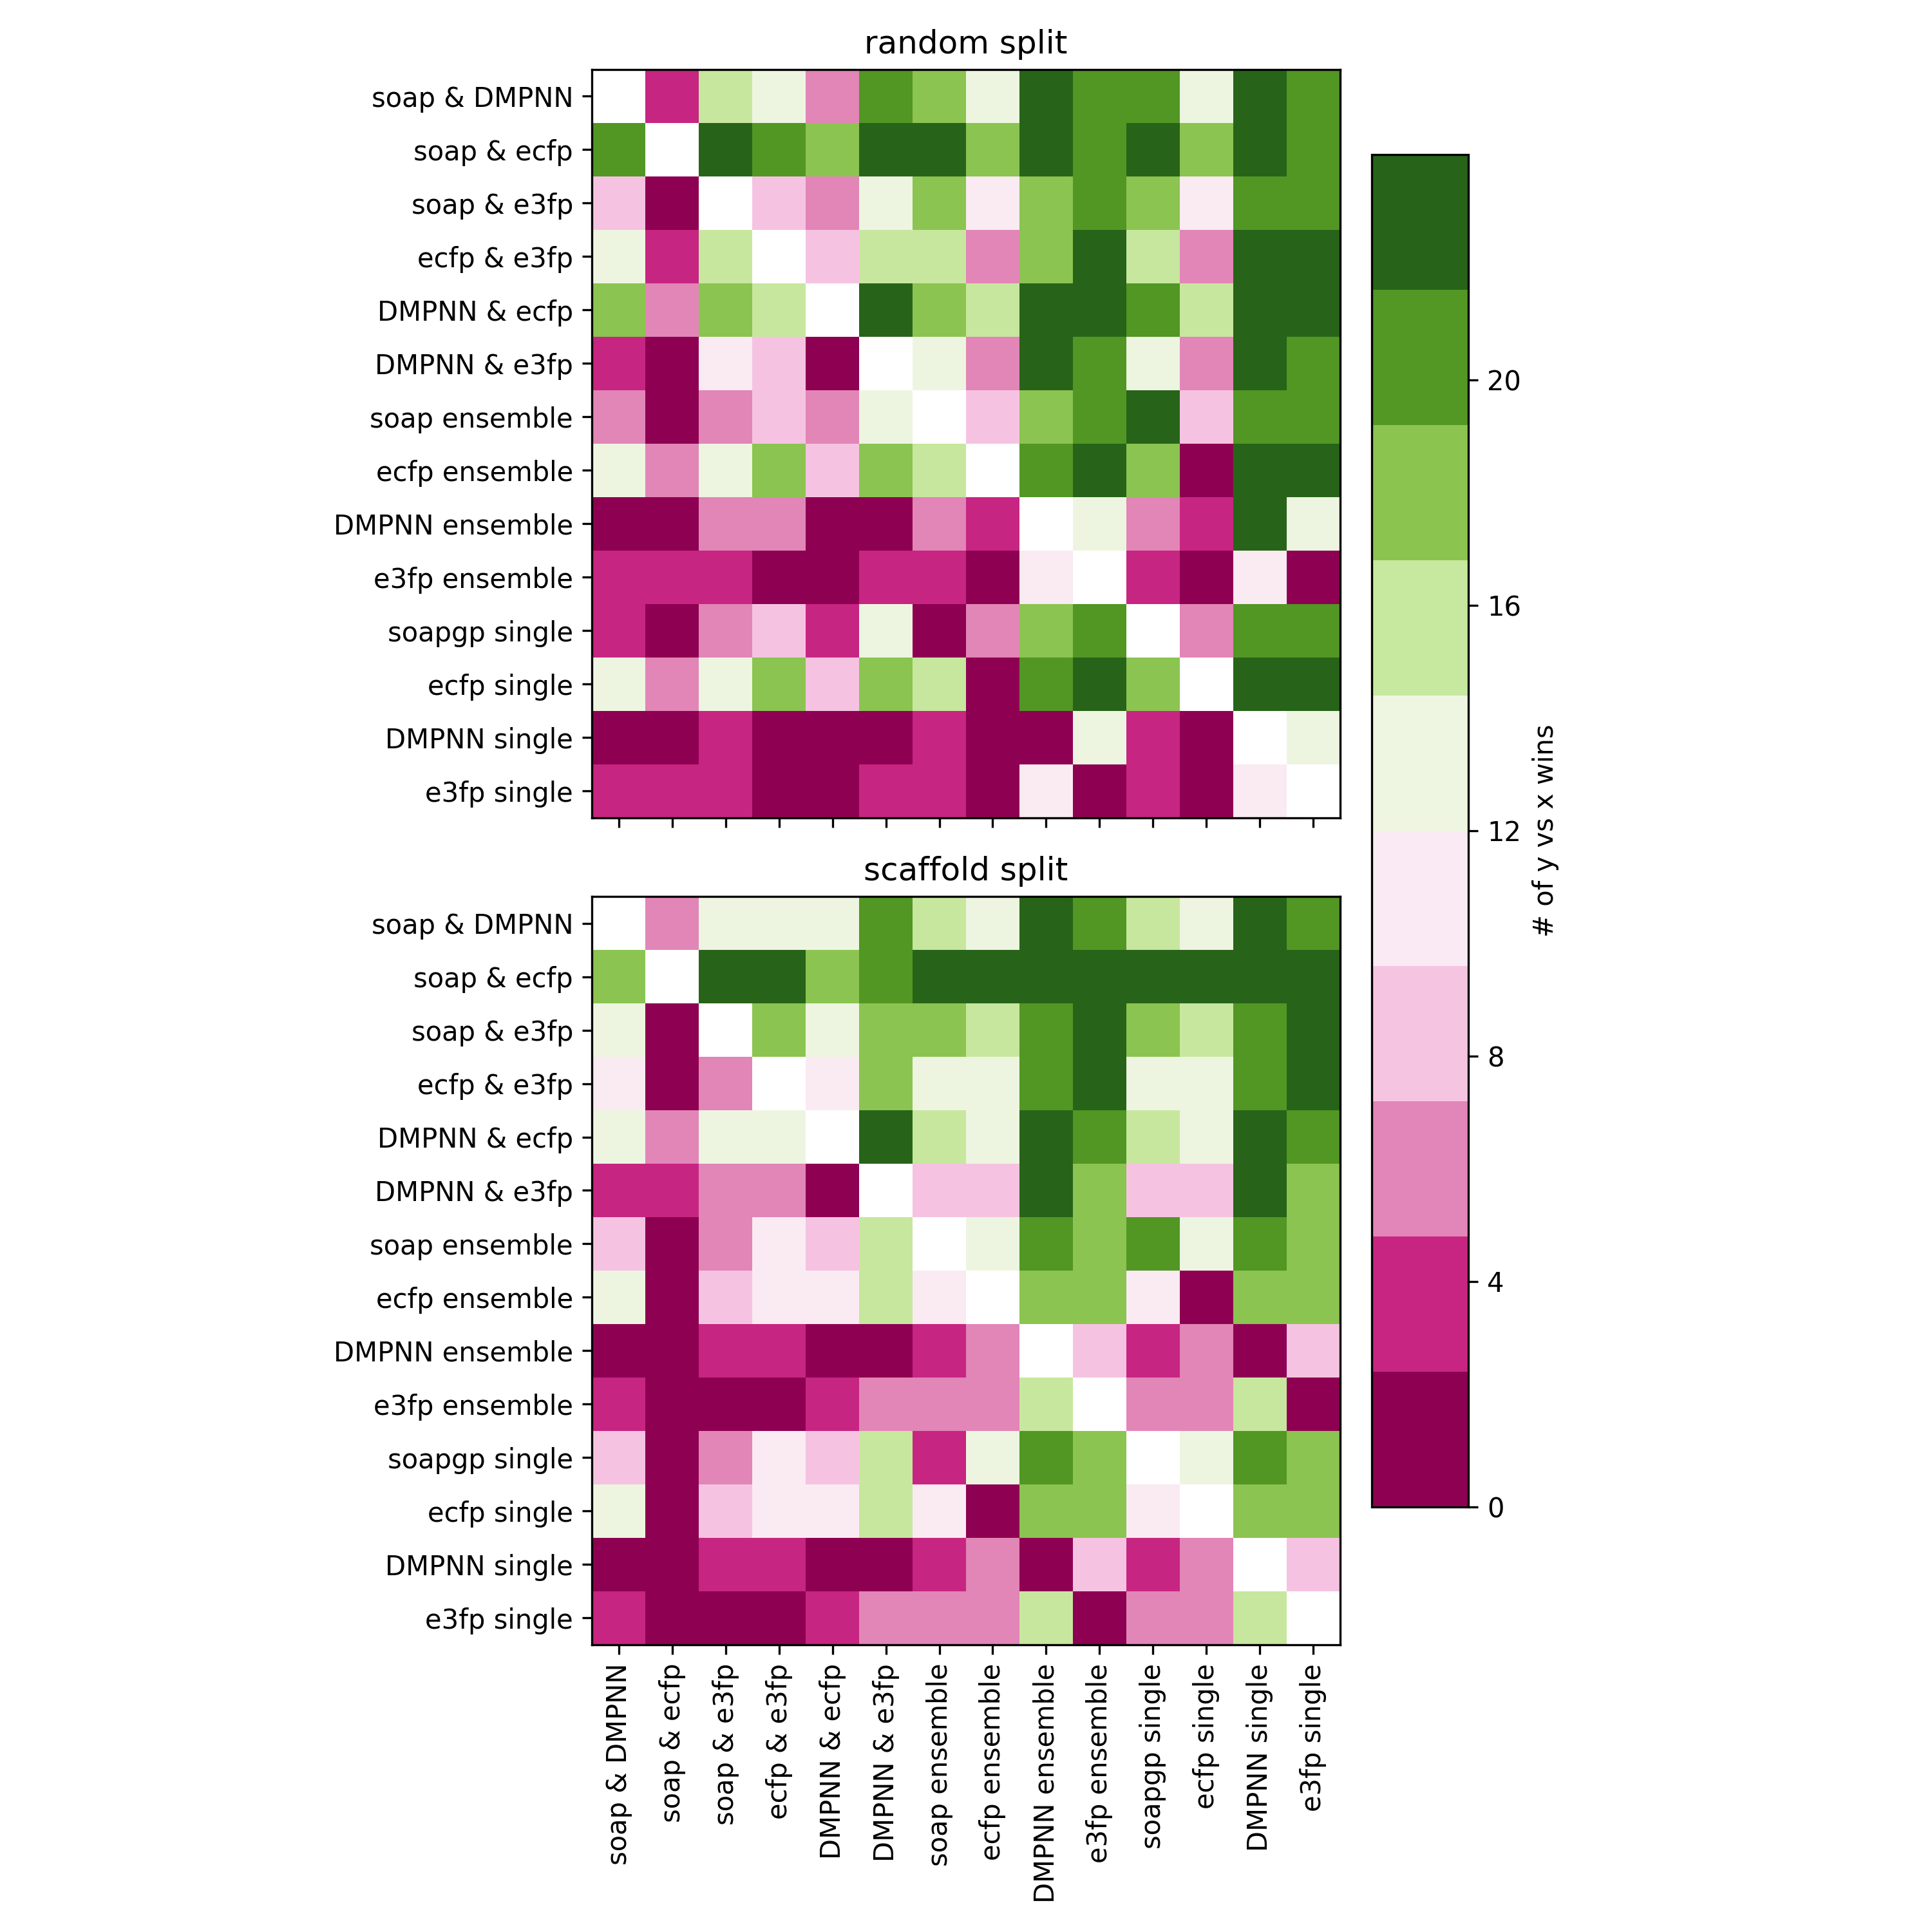
\includegraphics[width=\textwidth]{Chapter2/Figs/ensemble_wins.png}
\caption{\label{fig:ensemble_mat} Ensembling diverse representations is superior to ensembling similar representations regardless of model architecture. Green/red colour intensity indicates the number of tasks out of 24 in which the ensemble on the y-axis has a better/worse RMSE than the ensemble on the x-axis.}
\end{figure}

\subsection{Ensembling Representations}
Although we have showcased the competitive capabilities of SOAP-GP, we do not suggest that SOAP-GP should become the new paradigm in cheminformatics QSAR, nor indeed that any sole representation/model should be. From our dataset of 24 targets alone we can already observe that model performance can vary substantially and that it is hard to know a priori which model would do best. We argue that this is the case generally in bioactivity prediction and it is unhelpful to solely rely on any particular `state of the art' model or molecular featurisation for QSAR modelling.

Our argument is specifically for the learning of accurate ligand-binding affinity. When conducting a vast virtual screen of a molecular library or attempting to classify activity from a large high-throughput-screen, practical considerations such as time constraints and the memory scaling behaviour of models should dictate the choice of model. However, exact IC50-accuracy activity data essentially never exceeds $N=10^{4}$ in size \cite{Cherkasov2014QSAR}, and in this regime computational constraints are typically minor compared to demands on predictive performance.

In this scenario, a straightforward way to achieve improved performance is to combine QSAR models in an ensemble learning approach where the predictions from several models are averaged to give better results \cite{Sagi2018ensemble}. Such an approach is only successful if there is sufficient diversity such that each model captures trends in the dataset that are neglected by the others. The power of model ensembling lies not merely via the principle of `strength in numbers', but `strength in diversity'.

Model ensembling in QSAR has not been well-explored, and we propose that as a general principle it is important to include a diversity of representations in the ensemble, as opposed to ensembling different model architectures on the same representation. Unlike the conventional applications of machine learning, chemistry possesses an vast richness of featurisations and we should take advantage of this fact. Models trained on hybridization states and stereochemistry will capture distinct effects from those trained using conformational shapes, and these differences are much more significant than the particular architecture that is employed.

We demonstrate this by comparing the performance of ensembles with diverse representations pairwise against equivalently-sized ensembles that utilise the same features (Fig~\ref{fig:ensemble_mat}), as well as only single non-ensembled models. It can be seen that ensembling diverse representations almost always outperforms ensembling the same representation, which in turn tends to be better than the single models on their own. These differences are most accentuated in the scaffold split scenario. The best performing ensemble out of the possible combinations is an ensemble of SOAP-GP and ECFP-RF. This is not entirely surprising given that these were the two best-performing single models on their own, but it demonstrates that the trends learnt by the two models complement one another, that combining 2D topological information with precise 3D atomic features can push the predictive frontier of QSAR modelling.

\section{Outlook}
We described SOAP, a novel alignment-free 3D QSAR method which employs a GP model on the intermolecular similarity between local atomic environments featurized using SOAP descriptors. This model was compared with a 2D fingerprint-based random forest model, a 3D fingerprint-based GP, as well as a state-of-the-art graph convolutional neural network, DMPNN, on 24 IC50 regression tasks from ChEMBL. We showed that SOAP-GP is competitive with these on both random and challenging scaffold splits.

% There remains much scope for improving the performance of SOAP-GP, the most obvious starting point being the conformer generation for the three-dimensional molecular shape used to construct SOAP descriptors. In reality molecules exist in equilibria between multiple conformers, Boltzmann distributed by differing free energies due to electrostatic, steric, and orbital interactions. In the physical mechanism governing biological activity, some conformers may have much more favorable interaction with receptor binding sites than others, so there is strong reason to believe that it would be beneficial to account for this by include multiple conformers. Indeed, the effect of both the quality of the conformers generated, as well as going beyond single conformers has yet to be investigated.

% The competitive performance of SOAP-GP implies that the SOAP distance $d$ (Eq.~\ref{eq:distance}) is a better application-specific measure than fingerprint Tanimoto distances of the `distance' between molecules. While the use of SOAP for the embedding and visualisation of the abstract space spanned by atomic structures has been investigated in a materials science context~\cite{reinhardt2019ti02,bartok2017machine}, this has not yet been done specifically in the domain of medicinal chemistry on drug-like molecules. 

% Aside from improving performance, there is scope for future work in exploiting the uncertainty predictions from the GP using methods such as Bayesian Optimisation \cite{shahriari2016bo} to perform active learning. Being able to efficiently sample chemical space in order to search for molecules with optimal properties remains a difficult challenge in drug discovery.

The success of SOAP-GP in modelling ligand-protein binding affinity suggests that many other atomic/structural descriptors from the field of materials science, as well as the particular models that utilise those descriptors for the purpose of predicting quantum energies, have the potential to also be useful in QSAR modelling.

That being said, we believe that it is unrealistic to expect any single descriptor or model to be the best for any particular QSAR task. Thus, ensembling different models is the most principled way of conducting QSAR modelling in general. We further argue that ensembling models with diverse representations is fundamentally more important than ensembling diverse model architectures, and  demonstrate this by comparing the pairwise performance of equivalently sized ensembles with/without diverse representations. We find that ensembles with diverse representations outperform those with the same representation, and that SOAP-GP combined with ECFP-RF is by far the best performing model, showcasing the power of combining 2D and 3D features in capturing information relevant to predicting binding affinity.

Although much research is done on continually developing novel and improved QSAR models in a competitive basis, by instead taking a collaborative approach and complementing models with one another to exploit feature-rich chemistry, sizeable performance gains can also be achieved.

\renewcommand{\arraystretch}{1.0}